\documentclass[a4paper,12 pt,oneside]{report}
\usepackage{mystyle}
\usepackage{titling}
\graphicspath{{figures/}}

% \title{Ενσωμάτωση μηχανισμών caching,\\
% observability και self-healing στην υποδομή διαχείρισης\\
% δεδομένων ΙοΤ της πλατφόρμας Nostradamus}

\begin{document}

\begin{titlepage}

	% AUTH Logo and University Info
	\noindent
	\begin{minipage}[c]{0.3\textwidth}
		
\includegraphics[width=\linewidth]{./images/title/authLogoTr.jpg}
	\end{minipage}
	\hfill
	\begin{minipage}[c]{0.65\textwidth}
		\raggedright
		\large Αριστοτέλειο Πανεπιστήμιο Θεσσαλονίκης \\
		Πολυτεχνική Σχολή \\
		Τμήμα Ηλεκτρολόγων Μηχανικών $\&$ \\ Μηχανικών Υπολογιστών\\
		\normalsize{Τομέας Ηλεκτρονικής και Υπολογιστών} \\[5cm]
	\end{minipage}

	\vspace{1.5cm}

	\begin{center}
		\Large \textbf{Διπλωματική Εργασία} \\[0.8cm]

		\rule{350pt}{2pt} \\[0.6cm]

		{\fontsize{20.26pt}{1em}\selectfont
		Αρχιτεκτονική ενίσχυση
		αγροτικών IoT συστημάτων
		πραγματικού χρόνου
		}
		\rule{350pt}{2pt} \\[2cm]

		% Author
		\begin{minipage}[t][4cm][t]{0.45\textwidth}
			\raggedright
			\large
			\textit{Επιμέλεια:} \\
			Δημήτριος Ντέντας \\
			ΑΕΜ: 10446
		\end{minipage}%
		\hfill
		% Supervisors
		\begin{minipage}[t][4cm][t]{0.45\textwidth}
			\raggedleft
			\large
			\textit{Επίβλεψη:} \\
			Παναγιώτου~Κωνσταντίνος \\
			Γιώργος~Σιαχάμης
		\end{minipage}

		\vspace{2cm}

		\begin{center}
			{\large Θεσσαλονίκη, Ιανουάριος 2026}
		\end{center}
	\end{center}
\end{titlepage}

% \title{}
% \author{Δημήτριος Ντέντας}

% \date{\today}

\sloppy

% \maketitle
\tableofcontents

\newevenside
\pagenumbering{arabic}

\chapter{Εισαγωγή}


\chapter{Επισκόπηση της Ερευνητικής Περιοχής}

Στη σύγχρονη γεωργία, ένας δυσλειτουργικός αισθητήρας που περνά απαρατήρητος για ώρες μπορεί να οδηγήσει σε αποτυχημένο πότισμα ή καταστροφή καλλιεργειών. Αυτό το ενιαίο σημείο αποτυχίας αναδεικνύει την ανάγκη για αυτόνομα, ανθεκτικά και παρατηρήσιμα συστήματα σε κλίμακα. Η ανάγκη αυτή εναρμονίζεται με τον οδικό χάρτη (Roadmap) προς ανθεκτικά Κυβερνοφυσικά Συστήματα (CPS) που περιγράφεται από τους Ratasich et al. \cite{iotcps}, οι οποίοι δίνουν έμφαση στην ανίχνευση ανωμαλιών κατά τη διάρκεια λειτουργίας, στην απομόνωση σφαλμάτων και στην αυτοΐαση σε δυναμικά Internet of Things (IoT) περιβάλλοντα.

Οι συσκευές IoT παράγουν, σε πραγματικό χρόνο, μεγάλου όγκου δεδομένα, είτε σε μορφή χρονοσειράς, είτε ως ιστορικά δεδομένα \cite{rtiotevents}. Επομένως, η κλίμακα αυτή αποτελεί βασική αιτία εμφάνισης προβλημάτων και αστοχιών. Ωστόσο, για να εξασφαλιστεί η ομαλή λειτουργία των κρίσιμων υποδομών ενός νευραλγικού τομέα, όπως η γεωργία, οφείλουμε ως μηχανικοί να παρέχουμε λύσεις για τον παραγωγό και κατά συνέπεια για τον πολίτη, που εξασφαλίζουν τόσο την ποιότητα, όσο και την αναμενόμενη ποσότητα των αγροτικών προιόντων. Σε χώρες όπως η Ελλάδα, όπου η οικονομία και η αυτονομία, έγκεινται σε μεγάλο βαθμό στη γεωργική παραγωγή, η αξιοποίηση των τεχνολογιών πραγματικού χρόνου αποτελεί κρίσιμο παράγοντα για τη διασφάλιση της βιωσιμότητας και της αποδοτικότητας του πρωτογενούς τομέα. Η ανάπτυξη καινοτόμων υποδομών που ενσωματώνουν σύγχρονες τεχνολογίες όπως το \textit{Apache Kafka} για επεξεργασία σε πραγματικό χρόνο προσφέρει τη δυνατότητα συνεχούς παρακολούθησης, έγκαιρης παρέμβασης και λήψης αποφάσεων βασισμένων σε δεδομένα. Έτσι, ενισχύεται η ανθεκτικότητα του αγροδιατροφικού τομέα απέναντι στις προκλήσεις της εποχής, όπως η κλιματική αλλαγή, οι μεταβολές στη ζήτηση και η ανάγκη για βιώσιμη διαχείριση πόρων.

Σε κρίσιμες εφαρμογές, όπως η αγροδιατροφή, η διατάραξη στη ροή δεδομένων ή στη λήψη των αποφάσεων μπορεί να οδηγήσει σε σπατάλη τροφίμων, οικονομική απώλεια ή επισιτιστική ανασφάλεια. Σύμφωνα με τους Callo και Mansouri \cite{foodsec}, η ανθεκτικότητα των παγκόσμιων δικτύων διανομής τροφίμων εξαρτάται από την δυνατότητα των πληροφοριακών συστημάτων να ανταπεξέρχονται σε γεωπολιτικές ή υγειονομικές κρίσεις μέσω μηχανισμών ευελιξίας και προσαρμογής. Αυτό σημαίνει πως σε ότι αφορά σε αντίστοιχα συστήματα, στα οποία βασίζεται ο πλυθησμός (και η οικονομία) μιας χώρας, η αρχιτεκτονική που χρησιμοποιείται θα πρέπει να είναι άρτια, μελετημένη, αλλά και να εξασφαλίζει την ομαλή και συνεχή λειτουργία τους.

Οι σύγχρονες cloud-native τεχνολογίες παρέχουν τα εργαλεία και τα πρότυπα για την υλοποίηση τέτοιων χαρακτηριστικών, και την πρόληψη των προαναφερθέντων επιπτώσεων. Μέσω συνεχόμενης παρατήρησης ορισμένων μετρικών (\textit{Observability}), αλλά και ειδοποιήσεων σε κρίσιμες περιπτώσεις (\textit{Alerting}), μπορεί είτε να επανορθωθεί η ομαλή λειτουργία του συστήματος αυτόματα, είτε να ενημερωθεί ο αρμόδιος για την επανόρθωση χειριστής. Η ενσωμάτωση εργαλείων όπως το Prometheus σε cloud-native μικροϋπηρεσίες έχει ήδη αποδειχθεί αποτελεσματική σε εφαρμογές πραγματικού χρόνου, παρέχοντας κρίσιμη τηλεμετρία και αυτόματες ενέργειες ανάδρασης \cite{iotmonitoring}.

Βάσει της μελέτης των Sharma et al. \cite{iotagriculture}, αναδεικνύεται η ολοένα αυξανόμενη σημασία της χρήσης IoT τεχνολογιών στον τομέα της γεωργίας ακριβείας, όπου η αξιοποίηση αισθητήρων για την παρακολούθηση παραμέτρων όπως η υγρασία, η θερμοκρασία, η αγωγιμότητα και τα επίπεδα θρεπτικών συστατικών του εδάφους (NPK), επιτρέπει την ακριβή λήψη αποφάσεων σε πραγματικό χρόνο. Η προσέγγιση αυτή ευθυγραμμίζεται με την ανάγκη για ευέλικτες, αποκεντρωμένες υποδομές λήψης αποφάσεων, οι οποίες υποστηρίζονται από μηχανισμούς edge analytics και cloud ενορχήστρωσης. Στο πλαίσιο αυτό, η μελέτη των Akhtar et al. \cite{edgeagriculture} τονίζει τη σημασία της ενσωμάτωσης του edge computing για την επεξεργασία δεδομένων από αισθητήρες σε πραγματικό χρόνο, επιτρέποντας την αξιολόγηση του εδάφους και την παρακολούθηση ρύπων με μεγαλύτερη αποτελεσματικότητα. Υποστηρίζει, επιπλέον, πως η ενσωμάτωση τεχνικών μηχανικής μάθησης στην αλυσίδα επεξεργασίας των δεδομένων, όπως η αυτόματη πρόβλεψη της καταλληλότητας του εδάφους για συγκεκριμένες καλλιέργειες, ενισχύει την αξία των IoT συστημάτων και απαιτεί αρχιτεκτονική σχεδίαση που υποστηρίζει δυναμική ανάλυση και διαλειτουργικότητα. Τα ευρήματα αυτά ενισχύουν την άποψη ότι η αρχιτεκτονική ενός ανθεκτικού IoT συστήματος στον αγροδιατροφικό τομέα πρέπει να υποστηρίζει συνεχές monitoring, on-device προεπεξεργασία και ασφαλή, επεκτάσιμη μετάδοση δεδομένων, προκειμένου να επιτευχθεί πλήρης αυτοματοποίηση και ευστάθεια λειτουργίας σε ετερογενή, διασυνδεδεμένα περιβάλλοντα πεδίου.

Με στόχο, λοιπόν, την αρχιτεκτονική ενίσχυση του συστήματος \textit{Nostradamus} προτείνεται, ως απόρροια των παραπάνω μελετών, η ενσωμάτωση μηχανισμών caching, observability και self-healing. Παρότι υπάρχουν επιμέρους τεχνολογίες που προσφέρουν τέτοιες δυνατότητες, η υιοθέτησή τους σε πραγματικές πολυεπίπεδες IoT πλατφόρμες συνοδεύεται από σημαντικές προκλήσεις. Στα κατανεμημένα συστήματα, η προσθήκη μιας νέας υπηρεσίας ή λειτουργικότητας συνοδεύεται συχνά από μη προβλέψιμες επιπτώσεις στην απόδοση του συστήματος, όπως αναφέρει επανειλημμένα ο Kleppmann \cite{kleppmanndda}. Αν και οι μηχανισμοί όπως το caching και το observability αποσκοπούν στην βελτίωση της εμπειρίας και της διαχειρισιμότητας, μπορούν, ως παράπλευρη συνέπεια, να οδηγήσουν σε αύξηση του latency ή της κατανάλωσης πόρων. Το φαινόμενο αυτό αποδίδεται στην πολυπλοκότητα των αλληλεπιδράσεων μεταξύ μικροϋπηρεσιών και την έλλειψη πλήρους visibility σε runtime επίπεδο.

Κατ’ επέκταση, η ερευνητική συνεισφορά εστιάζει όχι μόνο στην επιλογή σχετικών τεχνολογιών, αλλά κυρίως στη συνεκτική και δυναμική ενορχήστρωσή τους, με στόχο την επίτευξη αυτονομίας και διαχειρισιμότητας σε cloud-native κατανεμημένα περιβάλλοντα υψηλής πολυπλοκότητας, για την υποστήριξη αυτού του συστήματος πραγματικού χρόνου στο χώρο του \textit{food security}.


\chapter{Θεωρητικό Υπόβαθρο}

Η εξέλιξη των Κυβερνο-Φυσικών Συστημάτων (CPS) και των εφαρμογών IoT βασίζεται σε θεμελιώδεις αρχιτεκτονικές αρχές που συνδυάζουν την αποδοτική διαχείριση της φυσικής πληροφορίας με τις δυνατότητες της σύγχρονης υπολογιστικής τεχνολογίας. Σε αυτό το κεφάλαιο παρουσιάζονται τα βασικά αρχιτεκτονικά μοντέλα, οι μέθοδοι διασύνδεσης υποσυστημάτων και τα πρότυπα διαχείρισης δεδομένων που επικρατούν στα σύγχρονα CPS.

\section{Αρχιτεκτονικές CPS και Κατανεμημένα Συστήματα}

Τα CPS δομούνται τυπικά σε τρία επίπεδα: το \textbf{φυσικό επίπεδο} (sensing/actuation), το \textbf{επίπεδο δικτύου} (networking/communication) και το \textbf{κυβερνητικό ή υπολογιστικό επίπεδο} (cyber/computation). Το φυσικό επίπεδο περιλαμβάνει αισθητήρες και ενεργοποιητές, το δίκτυο μεταφέρει τα δεδομένα, ενώ το κυβερνητικό επίπεδο διαχειρίζεται την επεξεργασία, την ανάλυση και τη λήψη αποφάσεων.

Η σύγχρονη σχεδίαση CPS ακολουθεί τα παρακάτω αρχιτεκτονικά μοτίβα:

\begin{itemize}
	\item \textbf{Layered (στρωματοποιημένη) αρχιτεκτονική}: Διαχωρισμός φυσικών, δικτυακών και υπολογιστικών λειτουργιών, διευκολύνοντας τη διαλειτουργικότητα και τη συντήρηση.
	\item \textbf{Κατανεμημένη επεξεργασία}: Τα δεδομένα δεν συγκεντρώνονται υποχρεωτικά σε έναν κεντρικό κόμβο, αλλά επεξεργάζονται τοπικά (\textit{edge/fog computing}) ή υβριδικά, βελτιώνοντας την καθυστέρηση και την ανθεκτικότητα.
	\item \textbf{Event-driven και streaming αρχιτεκτονική}: Αντί της παραδοσιακής batch επεξεργασίας, τα δεδομένα ρέουν ως ακολουθίες γεγονότων (streams), επιτρέποντας την άμεση αντίδραση σε αλλαγές του περιβάλλοντος.
	\item \textbf{Μικροϋπηρεσίες (Microservices)}: Ανάπτυξη του λογισμικού σε μικρές, αυτόνομες υπηρεσίες με σαφή όρια ευθύνης και ανεξάρτητο κύκλο ζωής.
	\item \textbf{Loose coupling \& αναγνωσιμότητα}: Η επικοινωνία μεταξύ των υποσυστημάτων βασίζεται σε ασύγχρονα μηνύματα (π.χ. μέσω pub/sub patterns), διατηρώντας την αυτονομία και διευκολύνοντας την κλιμάκωση.
\end{itemize}

\section{Streams, Event-Driven και Batch vs Real-Time Processing}

Η \textit{ροή δεδομένων} (stream) ορίζεται ως η συνεχής αλληλουχία δεδομένων που παράγονται από αισθητήρες ή άλλες πηγές και διακινούνται ασύγχρονα εντός του συστήματος. Η \textbf{event-driven αρχιτεκτονική} επιτρέπει τη λήψη αποφάσεων ή την ενεργοποίηση ενεργειών αμέσως με την εμφάνιση ενός γεγονότος, κάτι που είναι κρίσιμο για εφαρμογές με απαιτήσεις απόκρισης σε πραγματικό χρόνο, όπως η γεωργία ακριβείας, το predictive maintenance, ή η αυτονομία ρομποτικών συστημάτων.

Σε αντίθεση, τα παραδοσιακά \textit{batch systems} επεξεργάζονται δεδομένα συγκεντρωτικά και περιοδικά, οδηγώντας σε υστέρηση που δεν είναι αποδεκτή για CPS με κρίσιμες λειτουργίες. Η υιοθέτηση stream processing (με αρχιτεκτονικές Lambda/Kappa) προσφέρει καλύτερη προσαρμοστικότητα και αυτονομία, ενώ μειώνει την καθυστέρηση λήψης αποφάσεων.

\section{Αρχιτεκτονικές Streams: Lambda και Kappa}

Οι δύο επικρατέστερες αρχιτεκτονικές για επεξεργασία ροών είναι:

\begin{itemize}
	\item \textbf{Lambda}: Συνδυάζει speed layer για άμεση επεξεργασία (με πιθανό μικρότερο accuracy) και batch layer για πλήρη ανάλυση με υψηλότερη ακρίβεια, υποστηρίζοντας τόσο real-time όσο και offline analytics.
	\item \textbf{Kappa}: Ενιαία προσέγγιση, όπου όλα τα δεδομένα αντιμετωπίζονται ως streams, απλοποιώντας τη διαχείριση και επανεπεξεργασία γεγονότων χωρίς ανάγκη ξεχωριστού batch υποσυστήματος.
\end{itemize}

Η επιλογή μοντέλου εξαρτάται από το αν προτεραιότητα δίνεται στην αμεσότητα ή στην αναλυτική επεξεργασία και από τη συνολική πολυπλοκότητα συντήρησης. Σε πρακτικό επίπεδο, υλοποιήσεις όπως το \textit{Apache Kafka} (messaging/stream log), \textit{Apache Flink} και \textit{Apache Spark} (stream processing) έχουν επικρατήσει ως τεχνολογικά standards, λόγω της ευελιξίας, αξιοπιστίας και δυνατότητας διασύνδεσης με άλλα υποσυστήματα.

\section{Διασύνδεση Υποσυστημάτων}

Για την αλληλεπίδραση πολλαπλών, ετερογενών υποσυστημάτων, υιοθετείται το \textbf{publish/subscribe} μοτίβο. Αυτό επιτρέπει την ασύγχρονη και χαλαρά συνδεδεμένη (\textit{loosely coupled}) επικοινωνία μεταξύ παραγωγών (\textit{publishers}) και καταναλωτών (\textit{subscribers}), διασφαλίζοντας την αυτονομία, την επεκτασιμότητα και τη δυνατότητα αλλαγών στην τοπολογία του συστήματος χωρίς κεντρικό συντονισμό.

Η ποιότητα υπηρεσίας (\textit{Quality of Service, QoS}) αποκτά ιδιαίτερη σημασία, καθώς καθορίζει το επίπεδο αξιοπιστίας στη διανομή μηνυμάτων, ειδικά σε περιβάλλοντα με ασταθή συνδεσιμότητα (π.χ. αγροτικά δίκτυα, βιομηχανικά IoT). Για ποιοτικά περιορισμένες συσκευές και low-power δίκτυα, πρωτόκολλα όπως το \textit{MQTT} προσφέρουν ελαφριά, αξιόπιστη και ασφαλή ανταλλαγή μηνυμάτων, ενισχύοντας την ανθεκτικότητα του συστήματος.

\section{Αποθήκευση, Consistency Models και Caching}

Η αποθήκευση δεδομένων σε CPS συνιστά αρχιτεκτονική πρόκληση λόγω του όγκου, της ταχύτητας παραγωγής και της ανάγκης για real-time προσπέλαση. Κατανεμημένα συστήματα βάσεων (NoSQL, wide-column stores) με replication και partitioning διασφαλίζουν διαθεσιμότητα και fault tolerance.

Η επιλογή consistency model (strong, eventual, causal) εξαρτάται από τις απαιτήσεις της εφαρμογής για ακρίβεια vs ταχύτητα και διαθεσιμότητα. Σε συστήματα που μπορούν να αντέξουν μικρές απώλειες ή προσωρινή ασυνέπεια, το eventual consistency αποτελεί πρακτικό συμβιβασμό.

Επισημαίνεται επίσης, ότι η χρήση \textit{in-memory caching} (π.χ. με Redis/Memcached) μειώνει δραστικά το latency για δεδομένα που προσπελαύνονται συχνά ή απαιτούν άμεση διαθεσιμότητα, με trade-offs σε αντοχή σε αποτυχίες (durability).

\section{Διαχείριση Υποδομής και Cloud-Native Patterns}

Η ανάπτυξη CPS σε cloud ή υβριδικά περιβάλλοντα απαιτεί αυτοματοποιημένη διαχείριση υποδομής και υπηρεσιών. Εδώ κυριαρχεί η χρήση πλατφόρμων όπως το Kubernetes, που υλοποιούν:

\begin{itemize}
	\item \textbf{Δηλωτική διαχείριση (declarative infrastructure)}: Η επιθυμητή κατάσταση του συστήματος ορίζεται μέσω configuration, και ο orchestrator διασφαλίζει ότι αυτή τηρείται.
	\item \textbf{Αυτόματη κλιμάκωση (auto-scaling), αυτοΐαση (self-healing)}: Προσθήκη/αφαίρεση pods, επανεκκινήσεις σε περίπτωση αποτυχιών, health checks.
	\item \textbf{Παρατηρησιμότητα (observability)}: Συλλογή μετρικών, logs, tracing και alerting, με ενδεικτικά εργαλεία Prometheus, Grafana, ELK/EFK stack.
	\item \textbf{Διαμοιρασμός πόρων (virtualization)}: Ευνοϊκή μεθοδολογία για την απομόνωση εφαρμογών και την καλύτερη αξιοποίηση του διαθέσιμου hardware μέσω εικονικών μηχανών ή containers.
	\item \textbf{Αυτοματοποιημένος έλεγχος με Kubernetes Operators}: Επέκταση του control plane του Kubernetes, με αρχές αυτοματοποιημένων συστημάτων ελέγχου για τη διαχείριση σύνθετων, κατανεμημένων εφαρμογών.
	\item \textbf{Service discovery, load balancing και secrets management}: Απαραίτητα για τη διασύνδεση μικροϋπηρεσιών και τη διατήρηση ασφάλειας και διαθεσιμότητας.
\end{itemize}

Έτσι, η υποδομή μεταμορφώνεται σε έναν ζωντανό οργανισμό που προσαρμόζεται διαρκώς στις απαιτήσεις του συστήματος και του περιβάλλοντος, προσφέροντας ευελιξία και ανθεκτικότητα χωρίς ανθρώπινη παρέμβαση. Με αυτόν τον τρόπο, περιορίζονται τα λάθη του ανθρώπινου παράγοντα, καθώς κρίσιμες λειτουργίες αυτοματοποιούνται και αναλαμβάνονται από το ίδιο το σύστημα.

\section{Συμπεράσματα Αρχιτεκτονικής}

Η επιτυχία ενός σύγχρονου CPS/IoT συστήματος εξαρτάται από την υιοθέτηση δοκιμασμένων αρχιτεκτονικών προτύπων, τη σαφή οριοθέτηση των στρωμάτων (sensing, networking, processing, storage, observability), και τη χρήση τεχνολογιών που υποστηρίζουν real-time streaming, fault tolerance, scalability, automation και ασφάλεια. Οι επιλογές σε επίπεδο εργαλείων (Kafka, Flink, Cassandra, Redis, Kubernetes, Prometheus, κτλ.) υλοποιούν στην πράξη τα θεμελιώδη design patterns που περιγράφηκαν σε αυτό το κεφάλαιο, αποτελώντας τη “γέφυρα” μεταξύ θεωρίας και εφαρμογής.


\chapter{Εργαλεία}

Τα Κυβερνο-Φυσικά Συστήματα (CPS) είναι συστήματα που αποτελούνται από ένα
φυσικό στοιχείο το οποίο ελέγχεται ή παρακολουθείται από ένα κυβερνητικό
(cyber) στοιχείο, έναν αλγόριθμο βασισμένο σε υπολογιστή. Με στόχο να
μετασχηματίσουν τον τρόπο με τον οποίο οι άνθρωποι αλληλεπιδρούν με τα μηχανικά
συστήματα, τα νέα έξυπνα CPS οδηγούν την καινοτομία σε διάφορους τομείς,
βασικός εκ των οποίων αποτελεί η γεωργία \cite{cps}. Η αρχιτεκτονική των CPS
βασίζεται σε τρία βασικά επίπεδα: το φυσικό επίπεδο (physical layer), όπου
καταγράφονται και παράγονται τα δεδομένα μέσω αισθητήρων· το επίπεδο δικτύου
(network layer), που εξασφαλίζει τη μεταφορά των δεδομένων· και το κυβερνητικό
ή υπολογιστικό επίπεδο (cyber layer), όπου λαμβάνονται αποφάσεις βάσει των
εισερχόμενων δεδομένων. Η συνύπαρξη αυτών των στρωμάτων σε ένα κοινό σύστημα
καθιστά τα CPS ιδιαίτερα κατάλληλα για εφαρμογές που απαιτούν χαμηλή
καθυστέρηση, αξιοπιστία και αυτονομία. Όπως προαναφέρθηκε, στο πεδίο της
γεωργίας ακριβείας, τα CPS διαδραματίζουν καθοριστικό ρόλο, καθώς συνδυάζουν
αισθητήρες πεδίου, μηχανισμούς ελέγχου άρδευσης, και αλγορίθμους πρόβλεψης
βασισμένους σε δεδομένα για να εξασφαλίσουν βέλτιστες συνθήκες καλλιέργειας. Οι
τεχνολογίες αυτές επιτρέπουν τη δυναμική λήψη αποφάσεων, μειώνουν τις απώλειες
και αυξάνουν την αποδοτικότητα σε όλα τα στάδια της παραγωγής.

Για να επιτευχθεί όμως η πλήρης δυναμική των CPS, απαιτούνται ισχυρές υποδομές
διασύνδεσης και διαχείρισης δεδομένων. Εδώ εντάσσεται η ανάγκη για αξιόπιστες
messaging πλατφόρμες, όπως το Apache Kafka, που διασφαλίζουν την συνεχή και
αξιόπιστη ροή πληροφοριών ανάμεσα στα υποσυστήματα ενός CPS. Το Apache Kafka
αποτελεί ένα - πλέον - de facto πρότυπο για την υλοποίηση τέτοιων messaging
υποδομών, χάρη στη δυνατότητα του να αποθηκεύει τα μηνύματα σε μορφή καταγραφής
(log-based) \cite{kafkabdd}. Η αρχιτεκτονική του Kafka ενδείκνυται ιδιαίτερα
για περιβάλλοντα που απαιτούν real ή near-real time επεξεργασία γεγονότων,
καθώς παρέχει υψηλή διαθεσιμότητα, εγγυημένη διανομή μηνυμάτων και δυνατότητα
οριζόντιας κλιμάκωσης. Συγκριτικές μελέτες \cite{rtkafka} επιβεβαιώνουν ότι το
Kafka παρουσιάζει σημαντικό πλεονέκτημα σε όρους throughput και fault tolerance
σε σχέση με άλλες προσεγγίσεις, γεγονός που το καθιστά κατάλληλο για
απαιτητικές IoT εφαρμογές με αυξημένο όγκο και ταχύτητα δεδομένων.

Σε ένα σύστημα όπως το \textit{Nostradamus}, όπου η ροή των δεδομένων είναι
αδιάκοπη και εξελίσσεται σε πραγματικό χρόνο, η ταχεία εισαγωγή και εξαγωγή των
δεδομένων εκτιμάται, τόσο για λόγους απόδοσης όσο και για την ελαχιστοποίηση
της κατανάλωσης υπολογιστικών πόρων. Δοθέντος ενός συνόλου αισθητήρων
τοποθετημένων σε έναν αγρό, οι οποίοι παράγουν συνεχώς δεδομένα, ο κεντρικός
broker πρέπει να τα λαμβάνει ορθά και εντός λογικών χρονικών πλαισίων, ενώ
ταυτόχρονα να τα επεξεργάζεται χωρίς να καταπονεί το συνολικό σύστημα. Συνεπώς,
πρέπει να ληφθούν υπόψη τόσο η ποιότητα υπηρεσίας (Quality of Service - QoS)
της messaging υποδομής όσο και οι εγγυήσεις παράδοσης που αυτή προσφέρει. Στη
συγκεκριμένη εφαρμογή, η απώλεια ενός μεμονωμένου δείγματος αισθητήρα δεν
επηρεάζει σημαντικά τη συνολική ανάλυση, επομένως η πολιτική
"\textbf{at-least-once}" αποτελεί μια ασφαλή και επαρκή επιλογή. Οι Kreps et
al. \cite{kafkaoriginal} προσθέτουν, πως το Kafka σχεδιάστηκε εξαρχής με
γνώμονα το υψηλό throughput, αποφεύγοντας περίπλοκους μηχανισμούς όπως το
two-phase commit και υιοθετώντας πιο αποδοτικές λύσεις για περιπτώσεις όπου η
απώλεια μηνυμάτων είναι αποδεκτή.

Τα δεδομένα που εισάγονται στα topics του \textit{Kafka} επεξεργάζονται και
καταλήγουν είτε σε επόμενα topics για μετέπειτα ανάλυση, είτε απευθείας σε
αποθηκευτικά συστήματα. Ο τρόπος με τον οποίο πραγματοποιείται η εν λόγω
επεξεργασία οφείλει να είναι, εν γένει, σε πραγματικό ή σχεδόν πραγματικό
χρόνο, καθώς τα δεδομένα παράγονται και εισάγονται στο σύστημα σε συνθήκες
online ροής. Επομένως, εργαλεία όπως το \textit{Apache Flink}, τα οποία
παρέχουν native υποστήριξη για stream processing με χαμηλή καθυστέρηση,
καθίστανται ιδανικά για την υλοποίηση του ενδιάμεσου επιπέδου επεξεργασίας.

Το \textit{Flink} επιτρέπει τον ορισμό παραθύρων (windows) με βάση τον χρόνο
γεγονότος (event time), την υλοποίηση πολύπλοκων λειτουργιών (όπως filtering,
aggregation, enrichment), καθώς και την ενσωμάτωση με messaging και
αποθηκευτικά συστήματα, μεταξώ των οποίων και το \textit{Apache Kafka} και το
\textit{Apache Cassandra}. Επιπλέον, μέσω του μηχανισμού state management που
διαθέτει, διασφαλίζεται η αξιοπιστία της επεξεργασίας, ακόμη και σε περιπτώσεις
προσωρινών αποτυχιών. Η ενσωμάτωση του σε αρχιτεκτονικές τύπου CPS επιτρέπει τη
δημιουργία πραγματικά αντιδραστικών συστημάτων, τα οποία μπορούν να λαμβάνουν
αποφάσεις βάσει εξελισσόμενων δεδομένων, χωρίς να απαιτείται off-line
επεξεργασία ή χρονική υστέρηση.

Η αποθήκευση μεγάλου όγκου δεδομένων σε κατανεμημένα συστήματα βασίζεται -
κυρίως - σε βάσεις δεδομένων τύπου \textit{wide-column}, με το \textit{Apache
	Cassandra} να αποτελεί ένα από τα πιο διαδεδομένα και ώριμα συστήματα σε αυτόν
τον χώρο. Το Cassandra ακολουθεί το μοντέλο \textit{eventual consistency},
υποστηρίζει κατανεμημένη αποθήκευση με replication και partitioning, και έχει
σχεδιαστεί για \textit{write-heavy} εφαρμογές \cite{cassandrawp}. Σε
περιβάλλοντα IoT, όπου οι συσκευές παράγουν συνεχώς δεδομένα τηλεμετρίας (π.χ.
θερμοκρασία, τάση, ρεύμα) με υψηλή συχνότητα, η Cassandra μπορεί να
λειτουργήσει ως backend αποθήκευσης για ροές δεδομένων σχεδόν σε πραγματικό
χρόνο, διασφαλίζοντας υψηλή διαθεσιμότητα και συνεχή εγγραφή με χαμηλό latency.
Η προσέγγιση αυτή έχει εφαρμοστεί επιτυχώς σε σενάρια όπως η παρακολούθηση
φωτοβολταϊκών μονάδων μέσω Raspberry Pi \cite{iotcassandra}, όπου το σύστημα
συλλέγει και αποθηκεύει μετρήσεις αισθητήρων κάθε 15 λεπτά για περαιτέρω
ανάλυση και βελτιστοποίηση απόδοσης. Αντίστοιχες αρχιτεκτονικές υποδεικνύουν τη
σημασία της επιλογής αποθηκευτικού συστήματος που να ανταποκρίνεται τόσο σε
επιχειρησιακές ανάγκες χαμηλής καθυστέρησης όσο και σε απαιτήσεις αξιοπιστίας
και επεκτασιμότητας.

Στη συγκεκριμένη περίπτωση, η υψηλή απόδοση (high performance) της
\textit{Cassandra} σε συνδυασμό με την εύκολη και ελαστική επεκτασιμότητα
(elastic scalability), καθιστά το σύστημα ιδανικό για εφαρμογές πραγματικού
χρόνου με έντονη ροή δεδομένων. Η δυνατότητα προσθήκης ή αφαίρεσης κόμβων
(nodes) χωρίς διακοπή λειτουργίας επιτρέπει την ομαλή προσαρμογή στις
αυξομειώσεις φορτίου, επιτρέπωντας το self-healing, διατηρώντας παράλληλα
σταθερή τη χρονική απόκριση. Καθώς το σύστημα απαιτεί ταχεία επεξεργασία, άμεση
καταχώρηση και αξιόπιστη αποθήκευση δεδομένων αισθητήρων πεδίου, η επιλογή μιας
αρχιτεκτονικής βασισμένης στην \textit{Cassandra} εξασφαλίζει υψηλή
διαθεσιμότητα και ανθεκτικότητα σε αποτυχία. Το λειτουργικό όφελος που
προκύπτει από αυτήν τη σχεδίαση δεν είναι απλώς επιθυμητό αλλά κρίσιμης
σημασίας, ιδιαίτερα σε περιβάλλοντα με απαιτήσεις χαμηλού latency, συνεχούς
διαθεσιμότητας και γραμμικής επεκτασιμότητας.

Τελικός στόχος του συστήματος Nostradamus είναι η αξιοποίηση των αποθηκευμένων
και επεξεργασμένων δεδομένων σε εφαρμογές διεπαφής, ώστε οι χρήστες να μπορούν
να λαμβάνουν οπτικοποιημένη και άμεσα αξιοποιήσιμη πληροφόρηση σχετικά με την
καλλιέργειά τους. Οι κόμβοι της βάσης δεδομένων διαδραματίζουν κρίσιμο ρόλο
στην τροφοδότηση των εφαρμογών με δεδομένα σε πραγματικό χρόνο. Η ανάγκη για
άμεση προσπέλαση σε δεδομένα, ιδιαίτερα σε περιβάλλοντα όπου η εισροή
πληροφορίας είναι συνεχής και εν δυνάμει μαζική, καθιστά απαραίτητη τη χρήση
μηχανισμών προσωρινής αποθήκευσης (in-memory caching).

Στο πλαίσιο αυτό, τεχνολογίες όπως το \textit{Memcached} \cite{memcachedfb} και
το \textit{Redis} \cite{redisia} προσφέρουν σημαντικά πλεονεκτήματα, μέσω της
υλοποίησης γρήγορων και αποδοτικών μηχανισμών αποθήκευσης ζευγών κλειδιού-τιμής
(key-value pairs). Οι εν λόγω λύσεις συμβάλλουν ουσιαστικά στη μείωση του
χρόνου και του κόστους προσπέλασης σε δεδομένα που διαφορετικά θα απαιτούσαν
αναζήτηση στη βάση. Η βασική τους διαφοροποίηση εντοπίζεται κυρίως στο
αρχιτεκτονικό τους μοντέλο και στον τρόπο διαχείρισης της ταυτόχρονης
εκτέλεσης, με το \textit{Memcached} να βασίζεται σε multithreaded επεξεργασία,
ενώ το \textit{Redis} αξιοποιεί μοντέλο event loop.

Η ανάγκη για παρατηρησιμότητα, αποδοτική διαχείριση προσωρινών δεδομένων και
σταθερή ροή μηνυμάτων σε περιβάλλοντα με κατανεμημένη υπολογιστική λογική,
καθιστά την πλατφόρμα \textit{Kubernetes}, συχνά, απαραίτητο δομικό στοιχείο. Η
δυνατότητα αυτόματης επανεκκίνησης αποτυχημένω πόρων (self-healing), η
υποστήριξη οριζόντιας κλιμάκωσης (horizontal pod autoscaling) και η
ενσωματωμένη παρακολούθηση της κατάστασης των υπηρεσιών (liveness/readiness
probes), προσδίδουν λειτουργική ανθεκτικότητα και διατηρούν τη διαθεσιμότητα
του συστήματος σε υψηλά επίπεδα, ακόμη και σε συνθήκες έντονου φορτίου ή υλικών
αποτυχιών.

Πέραν της αυτοματοποιημένης διαχείρισης πόρων, το \textit{Kubernetes} παρέχει
μια ενιαία πλατφόρμα παρατηρησιμότητας. Μέσω της ενσωμάτωσης εργαλείων όπως το
\textit{Prometheus} για συλλογή μετρικών, το \textit{Grafana} για οπτικοποίηση
και το \textit{AlertManager} για την αποστολή ειδοποιήσεων, \cite{inframon} -
κοινώς τη \textbf{lingua franca} του \textit{observability} - ενισχύεται η
κατανόηση της δυναμικής συμπεριφοράς του συστήματος σε πραγματικό χρόνο. Η
εγγενής υποστήριξη μηχανισμών για service discovery, load balancing και
declarative configuration, επιτρέπει την ευέλικτη ανάπτυξη και τον συντονισμό
μικροϋπηρεσιών, διευκολύνοντας την επίτευξη στόχων υψηλής διαθεσιμότητας και
επεκτασιμότητας σε cloud-native περιβάλλοντα. Συνεπώς, υιοθετώντας αντίστοιχα
πρότυπα, μπορούν να προληφθούν ανεπιθύμητες καταστάσεις και να διασφαλιστεί η
διατήρηση της ομαλής λειτουργίας ακόμα και υπο συνθήκες υψηλής πολυπλοκότητας.


\chapter{Υλοποιήσεις}

Λόγω των επιχειρημάτων της προηγούμενης ενότητας, η πλατφόρμα του
\textit{Nostradamus} αναπτύχθηκε πάνω στην τεχνολογία \textit{Kubernetes}, για
\textit{cloud native} λόγους, αλλά και λόγω της εύκολης παρατηρησιμότητας. Με
αυτόν τον τρόπο, η υποδομή που στηρίζει το έργο καθίσταται υψηλά διαθέσιμη, ενώ
οποιεσδήποτε διαταραχές του συστήματος αντιμετωπίζονται και επιλύονται
αυτόνομα, χωρίς ανθρώπινη παρέμβαση. Λόγου χάριν, σε περίπτωση που ένας κόμβος
παρουσιαστεί ώς μη διαθέσιμος ή ένα \textit{container} (ένα κομμάτι κάποιας
εφαρμογής της πλατφόρμας) καταρρεύσει λόγω προσωρινής αστοχίας λογισμικού ή
υπερφόρτωσης πόρων, το σύστημα αναλαμβάνει την αυτόματη επανεκκίνηση του
σχετικού pod ή ακόμα και τη μετεγκατάστασή του σε διαθέσιμο κόμβο, εφόσον
κριθεί αναγκάιο. Η χρήση μηχανισμών όπως το \textit{livenessProbe} και
\textit{readinessProbe} διασφαλίζει ότι οι υπηρεσίες βρίσκονται πάντα σε
λειτουργική κατάσταση και είναι προσβάσιμες μόνο όταν είναι έτοιμες να
εξυπηρετήσουν αιτήματα.

Η επιλογή αυτής της αρχιτεκτονικής επιτρέπει την υλοποίηση κρίσιμων μηχανισμών
αυτοΐασης (\textit{self-healing}) και κλιμάκωσης, οι οποίοι είναι απαραίτητοι
για το περιβάλλον της γεωργίας ακρίβειας, όπου απαιτείται συνεχής διαθεσιμότητα
και άμεση απόκριση σε μεταβολές φορτίου ή αποτυχιών. Παράλληλα, μέσω της
παρατηρησιμότητας (\textit{observability}) που προσφέρει το οικοσύστημα του
\textit{Kubernetes}, όπως η ενσωμάτωση του \textit{Prometheus} και του
\textit{Grafana}, η πλατφόρμα αποκτά δυνατότητα \textit{real-time} επιτήρησης
μετρήσεων, ειδοποιήσεων και ιχνηλασιμότητας των συμβάντων (\textit{tracing}).

\section{Αρχιτεκτονική υποδομή}

Η αρχιτεκτονική υποδομής της πλατφόρμας σχεδιάστηκε, όπως προαναφέρθηκε, με
σκοπό τη μέγιστη επεκτασιμότητα, διαθεσιμότητα και ασφάλεια, αξιοποιώντας
σύγχρονες τεχνολογίες αυτοματισμού και \textit{containerization}. Το υπόβαθρο
της υλοποίησης βασίζεται στο \textit{Kubernetes}, το οποίο στο πλαίσιο αυτό
φιλοξενήθηκε σε περιβάλλον \textit{homelab}, αλλά η φύση του επιτρέπει την
εύκολη και ομαλή μετάβαση σε οποιοδήποτε \textit{cloud provider}. Επίσης,
εφαρμόστηκαν πρακτικές υποδομής ως κώδικα (\textit{Infrastructure as Code}) και
διαχείρισης μέσω \textit{GitOps}.

\subsection{Τοπολογία και ρόλοι κόμβων}

Η υποδομή αποτελείται απο έναν \textit{Kubernetes cluster} με διακριτούς τύπους
κόμβων:

\begin{itemize}
	\item{\textbf{Control plane nodes}: Υπεύθυνοι για τη λειτουργία
	      του \textit{API server}, του \textit{scheduler}, του \textit{controller
		      manager} και του \textit{etcd}}
	\item{\textbf{Worker nodes}: Εκτελούν τα\textit{pods} των εφαρμογών}
\end{itemize}

Ο διακριτός διαχωρισμός είναι θεμελιώδης για την αξιοπιστία και την ασφάλεια
του \textit{cluster}. Έτσι ο έλεγχος παραμένει απρόσβλητος από αστάθειες ή
σφάλματα που προκαλούνται απο εφαρμογές. Με τη σειρά του, το
\textit{controlplane} συνεχίζει να παρακολουθεί και να θεραπεύει pods, ακόμα
και όταν κάποιες εφαρμογές αποτυγχάνουν.

Τα πειράματα της παρούσας εργασίας έγιναν, λοιπόν, σε έναν \textit{Kubernetes
	cluster} φιλοξενούμενο σε περιβάλλον \textit{homelab}, συγκεκριμένα σε
\textit{enterprise server Dell Poweredge r630}. Χρησιμοποιώντας τεχνολογία
\textit{virtualization} όπως το \textit{Proxmox} ο \textit{server} τμήθηκε σε 5
\textit{virtual machines}, τα οποία αποτελούν τον \textit{cluster}, τα 3 εκ των
οποίων αφιερώθηκαν σε \textit{controlplane nodes} (περιττός αριθμός για λόγους
διατήρησης του \textit{quorum}), ενώ τα υπόλοιπα 2 \textit{virtual machines},
με περισσότερους υπολογιστικούς πόρους, καθιστούν τα \textit{worker nodes}.

\section{Ροή δεδομένων σε πραγματικό χρόνο}

\subsection{Πηγές ροής δεδομένων}

Η αξιόπιστη και χαμηλής καθυστέρησης επεξεργασία ροών δεδομένων σε περιβάλλοντα
γεωργίας ακρίβειας προϋποθέτει την ύπαρξη ποικίλων, ετερογενών πηγών δεδομένων
που παρέχουν συνεχή και διαχρονικά κρίσιμη πληροφορία σχετικά με τη φυσική
κατάσταση του αγροτεμαχίου και τις περιβαλλοντικές μεταβλητές. Η παρούσα
πλατφόρμα σχεδιάστηκε ώστε να ενσωματώνει και να επεξεργάζεται δεδομένα σε
πραγματικό χρόνο από πηγές δεδομένων όπως αισθητήρες θερμοκρασίας και υγρασίας
εδάφους ή μετρητές βροχόπτωσης και φωτεινότητας.

\subsection{Τεχνολογίες Streaming}

Στην προηγούμενη ενότητα παρουσιάστηκε το \textit{Apache Kafka} ως το βασικό
μέσο ενδιάμεσης επικοινωνίας μεταξύ των στοιχείων της πλατφόρμας. Σενάρια
\textit{streaming}, όπως αυτό της πλατφόρμας \textit{Nostradamus}, βασίζονται
στο \textit{Kafka} ως τον κεντρικό κόμβο του συστήματος, ο οποίος λειτουργεί ως
η κύρια <<πηγή αλήθειας>> για όλα τα υποσυστήματα. Κάθε γεγονός που συμβαίνει
στο σύστημα καταγράφεται αρχικά στο \textit{Kafka}, και στη συνέχεια κάθε
μικροϋπηρεσία εγγράφεται στο αντίστοιχο <<θέμα>> (\textit{topic}) ώστε να
λαμβάνει μόνο τα μηνύματα που της είναι απαραίτητα. Με αυτόν τον τρόπο
επιτυγχάνεται ο σαφής διαχωρισμός ανάμεσα στη ροή δεδομένων σε πραγματικό χρόνο
και στην κατανάλωση των μηνυμάτων. Συνεπώς, η σωστή σχεδίαση της υποδομής
συλλογής και μεταφοράς δεδομένων έως το \textit{Kafka} είναι κρίσιμη, καθώς από
εκεί και πέρα ο διαμοιρασμός τους στα υπόλοιπα υποσυστήματα γίνεται με απλό και
αποδοτικό τρόπο.

Για το \textit{deployment} του \textit{Kafka} στην πλατφόρμα επιλέχθηκε το
μοτίβο του \textit{Kubernetes Operator}, με στόχο την υψηλή διαθεσιμότητα, την
ανθεκτικότητα σε αστοχίες και την αυτοματοποιημένη διαχείριση του κύκλου ζωής
του συστήματος. Συγκεκριμένα, χρησιμοποιήθηκε ο \textit{Strimzi Kafka
	Operator}, ο οποίος παρέχει πλήρη αυτοματοποίηση στην εγκατάσταση, ρύθμιση,
κλιμάκωση και αναβάθμιση των brokers, καθώς και στη διαχείριση των
\textit{topics} και των \textit{users}. Με αυτόν τον τρόπο αξιοποιούνται τα
πλεονεκτήματα του Kubernetes, όπως η ευκολία κλιμάκωσης, η αυτόματη
αποκατάσταση υπηρεσιών και η συνεπής διαχείριση πόρων, εξασφαλίζοντας παράλληλα
σταθερή και αποδοτική λειτουργία της υποδομής ροών. Τέλος, ο \textit{operator}
αυτός επιτρέπει την διαχείριση της υποδομής του \textit{Kafka} μέσω
\textit{GitOps} πρακτικών, γεγονός που ευθυγραμμίζεται με τις υπόλοιπες αρχές
και πρότυπα σχεδίασης της παρούσας εργασίας.

Είναι πλέον καθιερωμένη πρακτική οι αισθητήρες και γενικότερα οι χαμηλής
κατανάλωσης μικροελεγκτές που χρησιμοποιούνται σε υποδομές \textit{IoT} να
αποστέλλουν τα μηνύματά τους μέσω του πρωτοκόλλου \textit{MQTT}, καθώς αυτό
εξοικονομεί ενέργεια και επιτρέπει αποδοτική μετάδοση δεδομένων. Για την
εισαγωγή των μηνυμάτων αυτής της μορφής στο \textit{Kafka} απαιτείται η ύπαρξη
μηχανισμού γεφύρωσης. Στο πλαίσιο αυτό, αξιοποιήθηκε αρχικά το \textit{Strimzi
MQTT bridge}.

Ωστόσο, η ενσωματωμένη υλοποίηση του \textit{Strimzi} δεν υποστηρίζει ασφαλή
μεταφορά μέσω \textit{MQTTs}, γεγονός που αποτελεί κρίσιμο ζήτημα για την
παρούσα πλατφόρμα, δεδομένου ότι οι αισθητήρες βρίσκονται σε εξωτερικά δίκτυα.
Για την επίλυση του προβλήματος, ενσωματώθηκε ένας \textit{EMQX broker}, ο
οποίος λειτουργεί ως ασφαλής πύλη (\textit{secure gateway}) μεταξύ των
εξωτερικών συσκευών και του \textit{Kafka}, παρέχοντας υποστήριξη για
κρυπτογράφηση και μηχανισμούς πιστοποίησης σύμφωνα με τις απαιτήσεις της
αρχιτεκτονικής. Παράλληλα, ο \textit{EMQX broker} παρέχει δυνατότητες
φιλτραρίσματος βάσει των εισερχόμενων \textit{MQTT topics} και αντιστοίχισης
(\textit{mapping}) αυτών σε \textit{Kafka topics}, ώστε να προωθούνται στο
\textit{Kafka} μόνο τα απαραίτητα μηνύματα και να διατηρείται συνεπής η
ονοματολογία και η δομή των θεμάτων στην πλατφόρμα.

\subsection{Παρατηρησιμότητα Streaming}

\subsection{Ανθεκτικότητα και ανοχή σε σφάλματα}

\section{Ένταξη πελάτη}

\begin{figure}[H]
	\centering
	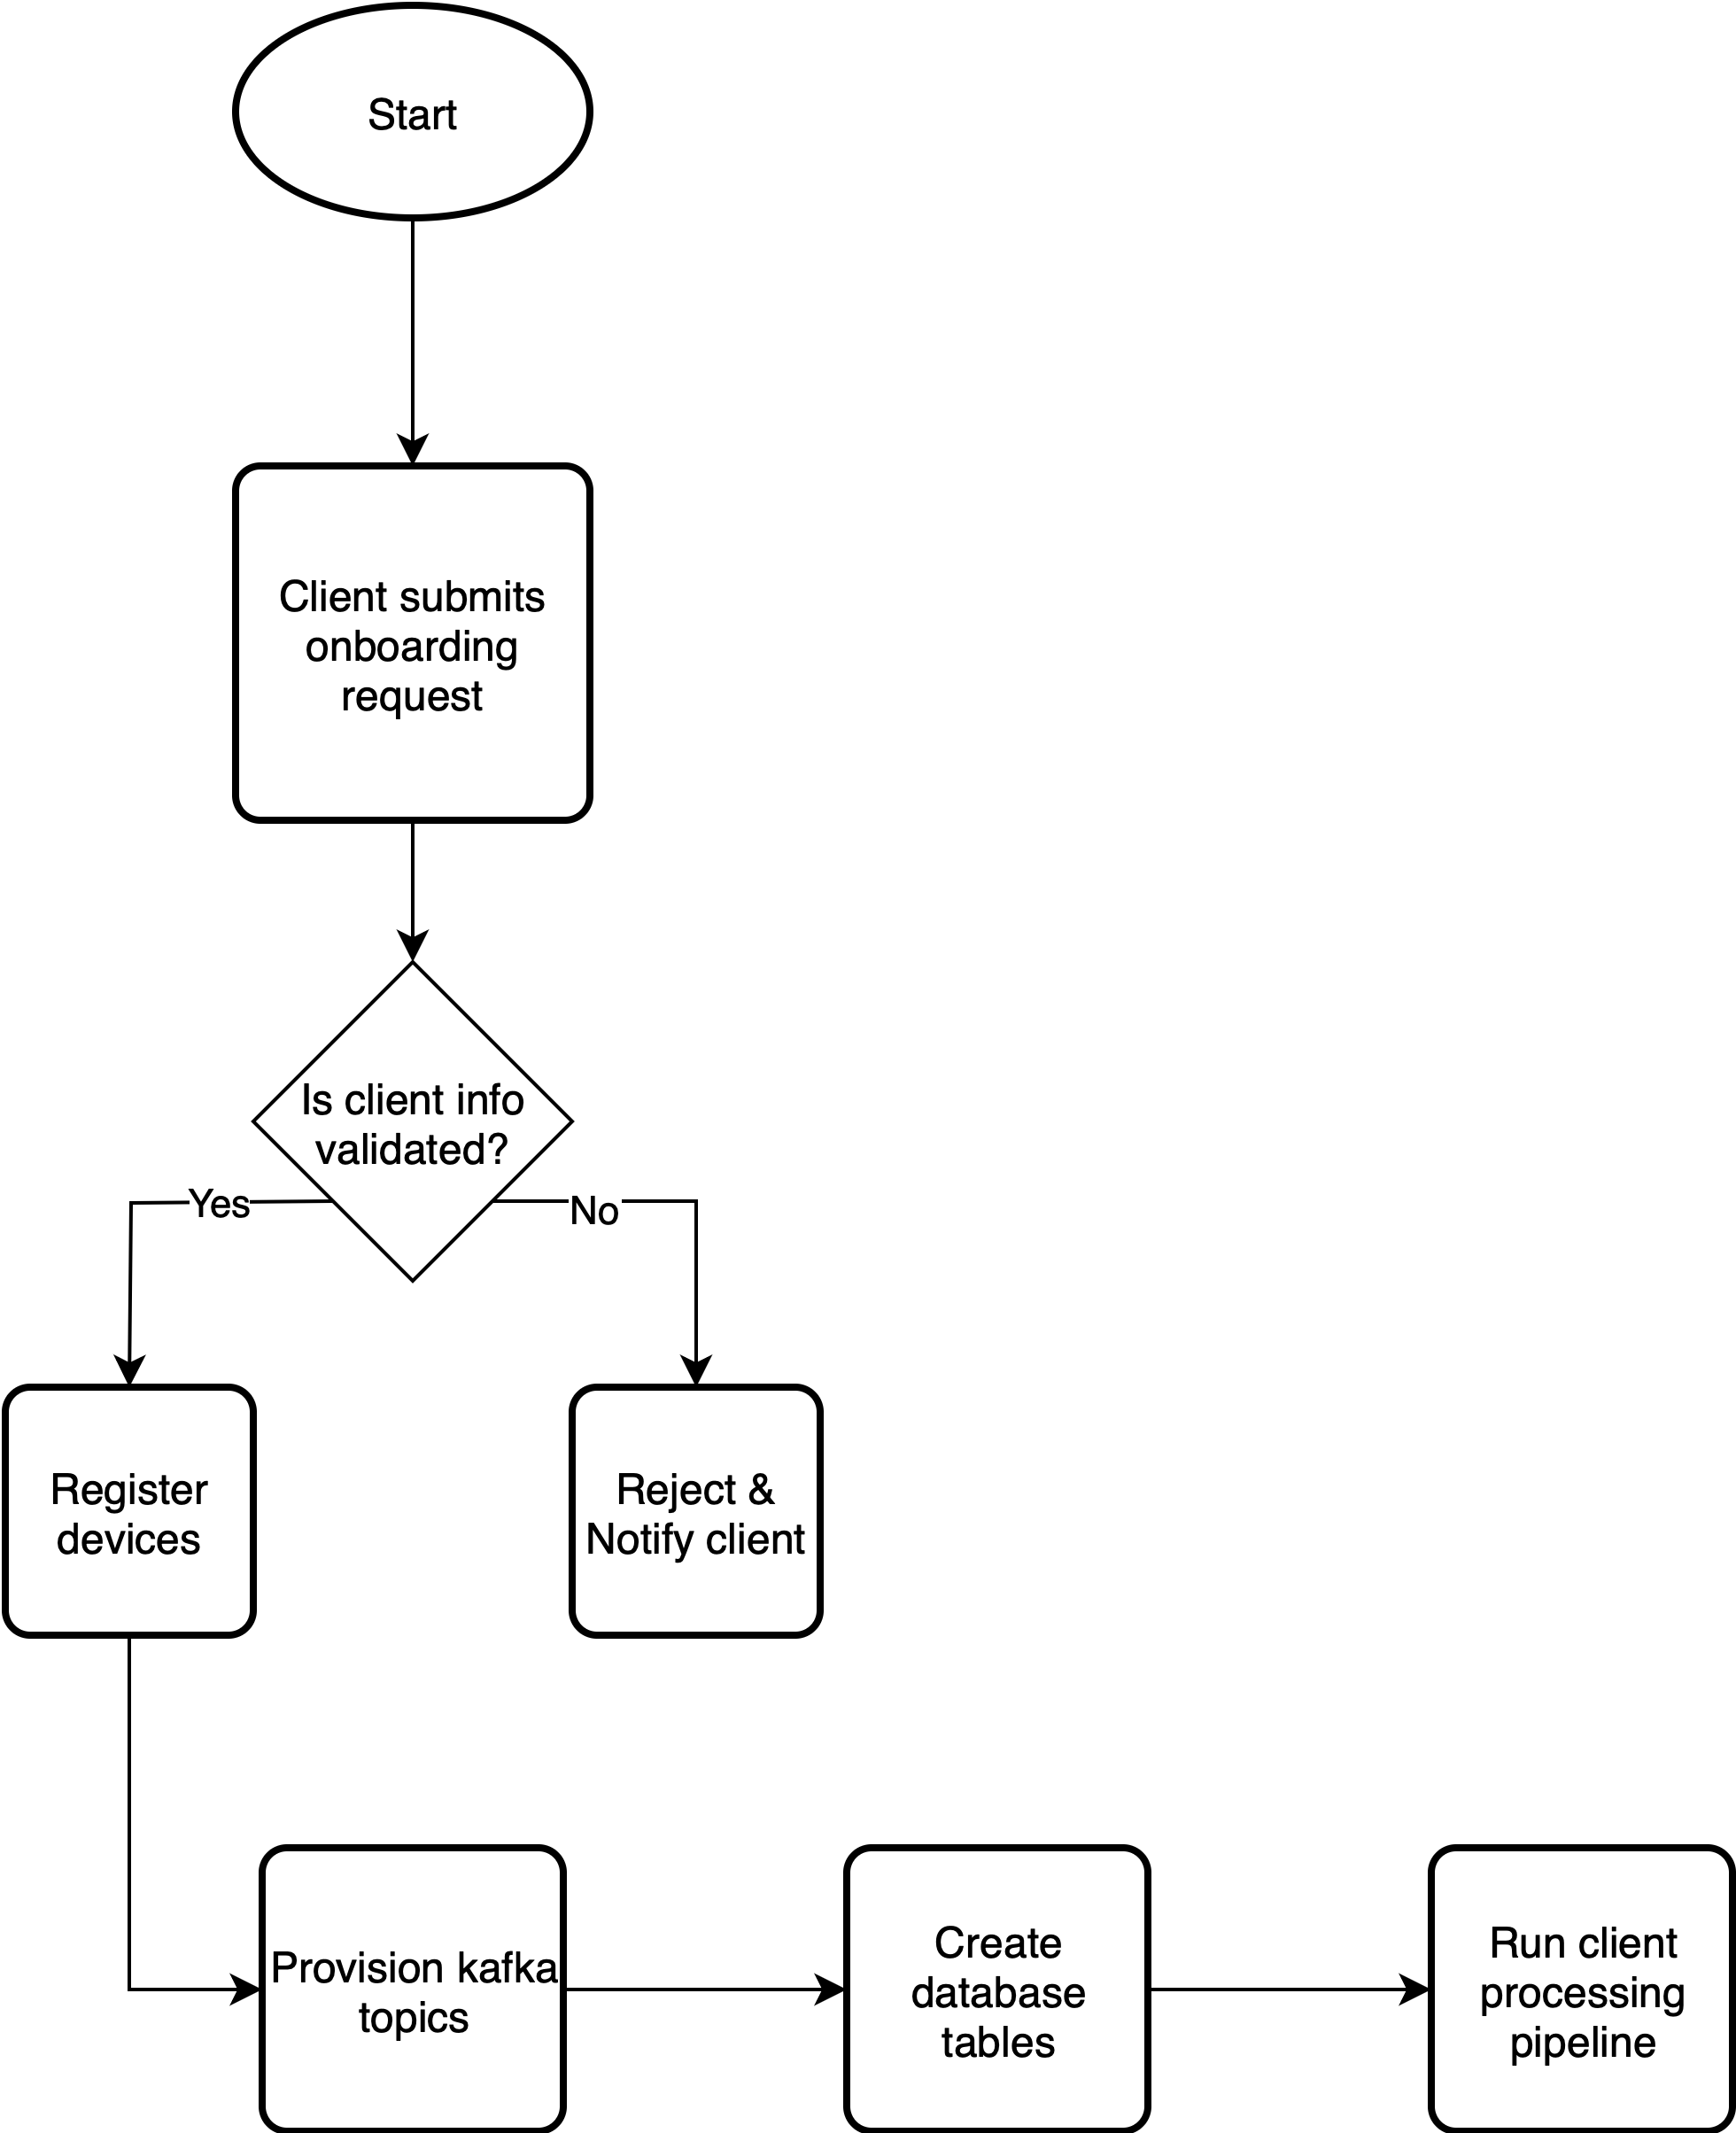
\includegraphics[width=0.7\textwidth]{client-onboarding-process}
	\caption{Διάγραμα δραστηριότητας για τη διαδικασία ένταξης νέου πελάτη}
	\label{fig:client-onboarding-activity}
\end{figure}


\chapter{Πειράματα}


\chapter{Συμπεράσματα}


\newevenside
\renewcommand{\bibname}{Βιβλιογραφία}
\bibliography{bib/references}

\end{document}
